% $Id: preview.tex,v 1.19 1998/06/22 08:07:00 ohl Exp $
%%%%%%%%%%%%%%%%%%%%%%%%%%%%%%%%%%%%%%%%%%%%%%%%%%%%%%%%%%%%%%%%%%%%%%%%


\NeedsTeXFormat{LaTeX2e}
\documentclass[11pt]{article}
\usepackage{amsmath,amssymb,amsthm}
\usepackage[margin=1.0in]{geometry}
\usepackage{amscd}
\usepackage{epsfig}
\allowdisplaybreaks
\setlength{\unitlength}{1mm}
%%%%%%%%%%%%%%%%%%%%%%%%%%%%%%%%%%%%%%%%%%%%%%%%%%%%%%%%%%%%%%%%%%%%%%%%
\makeindex
\begin{document}
\title{\bf {PURE DATA FOUNDATIONS OF MATHEMATICS}}
\author{%
  Saul Youssef%
  \hfil \\
  Department of Physics \\
  Boston University \\
  youssef@bu.edu\\
}
\maketitle
\begin{abstract}
This is an abstract.
\end{abstract}
%%%%%%%%%%%%%%%%%%%%%%%%%%%%%%%%%%%%%%%%%%%%%%%%%%%%%%%%%%%%%%%%%%%%%%%%

%%%%%%%%%%%%%%%%%%%%%%%%%%%%%%%%%%%%%%%%%%%%%%%%%%%%%%%%%%%%%%%%%%%%%%%%
\section{Introduction}

\section{Foundation}

     Any system of reasoning must necessarily have foundational concepts which are intrinsically understood, even before a first definition.  
In the case of type theories, for example,
there is no definition of `type' and in ZFC, there is no definition of `true', `false' or `set.'  In our case, we have one foundational undefined concept:  
the {\it finite sequence}.  We assume that finite sequences and `obvious' operations on finite sequences are understood\cite{obvious}.  On the other hand, logic, 
logical values and predicates will appear in coda as varieties of the central concept {\it data}, which is defined in terms of finite sequences as follows. 
\begin{itemize}
\item {\it Data} is a finite sequence of {\it codas}, and a {\it coda} is a pair of {\it data}. 
\end{itemize}
If $A$ and $B$ are data, there is a small natural {\it algebra of data} where $A\ B$ means the concatenation of $A$ and $B$ and $A:B$ means 
the coda formed by pairing $A$ and $B$.  For example, by the definition, the empty sequence of codas (written `$()$') is data.  Therefore,
the pairing of two empty sequences (written `$(:)$') is data, and, therefore, this sequence of three codas $(:) (:) ((:):(:))$ is also data.  
We refer to this as `pure data' since it is data `made from finite sequences of nothing.'   
We shall see that both data in the ordinary sense (bits, bytes, language expressions) and mathematical concepts such as variables, functions, definitions, 
logical values, categories, morphisms, types and theorems naturally appear as varieties of pure data with simple definitions expressed in the small algebra
of data with the concatenation and the colon operations.   Notationally speaking, the colon operation binds from the right first and binds 
less strongly than concatenation, so that $A:B:C$ means $(A:(B:C))$ and $A:B\ C$ means $(A:(B\ C))$ the length of $A$ as a finite sequence 
is denoted $|A|$.  

     In coda, the answers to mathematical questions come from an equivalence relation $=$, which is defined by a partial function from codas to data
called a {\it context}.  Given a context $\delta$, equality is defined by
\begin{equation} \label{eqn}
	A\ B = \delta(A)\ B = A\ \delta(B)
\end{equation}
\begin{equation} \label{eqn}
	A:B = \delta(A):B = A:\delta(B)
\end{equation}
for data $A$ and $B$ where the partial function $\delta$ has been extended to a function from data to data with identities.
Conceptually, relations are assumed until $\delta$ has the same properties as the identity function on data.  Within a given context, data $A$ is {\it empty} if $A=()$ and {\it invariant}
if $\delta(A)=A$.

     In coda, new definitions are added to a context as partial functions from codas to data.  We use a convention to guarantee that each such partial
function has it's own disjoint domain.  Let the {\it domain} of a coda $A:B$ be the data consisting of the first coda in the sequence $A$ and the empty
sequence if $A$ is empty.  A partial function mapping the all of the codas with a particular invariant domain to data is called a {\it definition}.  Definitions
can be added to a `valid' context if they do not clash, as guaranteed by the following. 

\newtheorem*{remark}{THE AXIOM OF DEFINITION}
\begin{remark}  The empty context is valid.  If $\delta$ is a valid context and $d$ is a definition, and if no coda is in
the domain of both $\delta$ and $d$, then the union of $\delta$ and $d$ is a valid context.
\end{remark}
\noindent As an axiomatic system, coda is complete at this point.  This is quite a contrast from, for instance, ZFC which has ten axioms 
even assuming predicate logic.  The reason for the simplification will become clear in the sections which follow.  In section 4, we show 
that coda already has an internal logic implicit in the structure as defined.  We adopt this logic for reasoning within coda, so we do not 
need axioms related to propositional or predicate logic.  In section 5, we show that coda also contains an internal language which can 
also be defined just as with any other definition.  The language has the unusual property that all byte sequences are valid syntax, 
so language and language syntax axioms are also not needed.  Axioms specifying valid ``rules of deduction'' are also not needed 
because deduction, proof, and computation in coda are all determined by the above data equality.  Each of these is a merely a data sequence $A_0=A_1=A_2=\dots=A_n$, 
deducing $A_n$ from $A_0$, computing $A_n$ starting with $A_0$ or proving that $A_0=A_n$, depending on one's point of view.  
Unlike type systems with a Curry-Howard correspondence, proof and computation are the same thing in coda. 

In the sections that follow, 
``data" and ``pure data'' are interchangeable terms and ``sequence'' will always mean a finite sequence unless otherwise indicated.  Since coda 
only has one axiom, we can refer to the Axiom of Definition as just ``the axiom.'' 

\section{Atoms}

      If we have invariant data $|D|\le 1$, we may, by the axiom, add a definition $(D A:B)\mapsto(D A:B)$ to context provided 
that $D$ has not already been used.  In this case, a coda $(D A:B)$ is called an {\it atom} for any $A$ and $B$.  
Data with at least one atom in it's sequence is called {\it atomic} data, and data which is equal to $()$ is called {\it empty} data. 
Equations (1) and (2) imply that empty data can not be equal to atomic data and the axiom implies that this fact remains 
true independent of future definitions.  We shall use the words `always' and `never' to refer to properties that are independent of 
future definition, so atomic data is `always' atomic, empty data is `always' empty and atomic data and empty data are `never' equal.  

    As we shall see in Section 4, the bifurcation between empty and atomic data is the basis for the internal logic of coda.  
Atoms are also the mechanism for defining permanent data such as bits, bytes and byte strings.   
Starting with the empty context, a first definition is suggested by the pure data examples above where pure data 
appears to be completely made from $()$ and $(:)$.  
This makes it clear that if we were to define $(:)\mapsto()$ it would cause all pure data to collapse and become equal to $()$.  
This suggests the alternative, mapping $(:)$, with invariant domain $()$, to itself, or, more generally defining $(:B)\mapsto(:B)$.  
This establishes that any $(:B)$ is an atom, and, since $()$ is invariant, it also establishes $(:)$ as a new invariant which can then be 
used as a domain for new definitions.  Continuing in this fashion, we define an invariant {\it 0-bit}, $((:):)$, and an invariant {\it 1-bit} $((:):(:))$.  
Atoms with a 0-bit domain are conventionally bit sequences and atoms with 1-bit domains are conventionally sequences of length 8 bit sequences.  
This makes ordinary byte sequences available as invariant names for new definitions.  For example, the definition $({\rm pass}\ A:B)\mapsto B$ 
maps all codas with invariant domain `pass' to their corresponding $B$, ignoring $A$ in this particular definition.  Depending on the situation, 
it is sometimes convenient to refer to `pass' as a `command,' thinking of $B$ as 
`input' and $A$ as `argument'.  Alternatively, `pass' can be thought of as a binary operator taking data $A$ and $B$ and producing data $B$. 
Typical examples of definitions are shown in Tables 1 and 2.  
\begin{table}
\begin{tabular}{ | l | l | l | }
Domain & Description & Action \\
\hline
pass & Pass input unchanged & (pass A:B)$\mapsto$ B \\
\hline
null & Empty data for any input & (null A:B)$\mapsto$ () \\
\hline
rev & Reverse the order of data & (rev : B)$\mapsto$ (), if B is empty \\
 &  & (rev : b)$\mapsto$ b, if b is an atom \\
 & & (rev : B C)$\mapsto$ (rev:B) (rev:A) \\ 
 \hline
 if & Conditional B & (if A:B) $\mapsto$ B, if B is empty \\
 & & (if A:B) $\mapsto$ (), if B is atomic. \\
 \hline 
 ap & Apply argument A to each input & (ap A : B)$\mapsto$ (), if B is empty \\
  & & (ap A : b)$\mapsto$ A:b, if b is an atom \\
  & & (ap A : B C)$\mapsto$ (ap A:B) (ap A:C) \\  
\hline
nat & The natural numbers & (nat : $n$)$\mapsto$ $n$ (nat\ :\ $n+1$) \\
\hline
def & Make a new definition & (def A:B)$\mapsto$ add definition (A $A'$:$B'$)$\mapsto$ B. \\
\hline 
\end{tabular}
\caption{\label{ }{\it Typical definitions in coda.  Each definition is a partial function from codas to data defined on  
codas with a specified domain.  When multiple actions are listed, the total action is defined by the first action 
where the left hand side pattern applies.}}
\end{table}
In addition to the approximately 50, very simple, pre-defined built in definitions, coda includes a definition (def A : B) which lets one 
add new definitions to a context provided that A is invariant and not already used in the context, according to the Axiom of Definition.
A particularly important and typical family of definitions are the {\it applications} such as {\bf ap} in Table 2.  These 
are simple combinatorial operations on sequences.  Taking finite sequences as understood, we presume that descriptions 
such as those in Table 2 are sufficient for a clear understanding of the meaning of these sorts of definitions.  Of course, further description and built in examples are available with the software, and the source code implementation of these is also always 
short and readable.  
\begin{table}
\begin{tabular}{| l  l  l | }
Schematic Coda & $\mapsto$ & Schematic Result \\
\hline
ap A:$b_1$ $b_2$ $b_3$ & $\mapsto$ & (A:$b_1$) (A:$b_2$) (A:$b_3$) \\
app $a_1$ $a_2$ $a_3$:B &  $\mapsto$ & ($a_1$:B) ($a_2$:B) ($a_3$:B) \\
ap2 $a$ $a_1$ $a_2$ $a_3$:B & $\mapsto$ & ($a$ $a_1$:$b_1$) ($a$ $a_2$:$b_2$) ($a$ $a_3$:$b_3$) \\
aps A:$b_1$ $b_2$ $b_3$ $b_4$ & $\mapsto$ & (A $b_1$:(A $b_2$ : (A $b_3$:$b_4$))) \\
apif A:$b_1$ $b_2$\dots & $\mapsto$ & $b_1$ (\dots if (A:$b_1$) is empty) $b_2$ (\dots if (A:$b_2$) is empty) \dots \\
\hline
\end{tabular} 
\caption{\label{ }{\it Built in definitions are typically combinatoric operations on data as finite sequences.  The `ap' series are variations on the 
idea of applying the `argument' A to `input' B, done in various ways.}}   
\end{table}

\section{Logic}

    In the framework of coda, items with mathematical meaning are represented as data.  This that mathematical 
questions will appear as questions about data.  Roughly speaking, mathematical questions will appear 
in the form 
\begin{itemize}
\item[] Is data $A$ equal to data $B$?
\end{itemize}
for some data $A$ and $B$.  
Since data equality itself is available as a definition, $A$, $B$, and the answer to the question should be encoded in the data $A=B$\cite{sugar}, 
including the logical meaning of the answer.  This suggests that `logic' in coda should be a suitable classification of 
data in general which matches our intuition and which is unchanging if definitions are added to context via the axiom.  
We already have such a classification via the disjoint classes of empty and atomic data, suggesting that we say that 
\begin{itemize}
\item data is {\it true} if it is empty, {\it false} if it is atomic and {\it undecided} otherwise. 
\end{itemize}
Table 3 shows examples of this classification, including coda versions of the familiar binary operations from classical logic.   
For instance, if data $A$ and $B$ are both either true or false then $({\bf xor}\ A:B)$ is $()$ for {\it true} and $(:)$ for {\it false} according to the standard truth
 table for the {\bf xor} operation.  On the other hand, if either $A$ or $B$ are 
undecided, the data $({\rm xor}\ A:B)$ has no definitions that apply.  In effect, $({\rm xor}\ A:B)$ `waits' until both $A$ and $B$ are defined enough to have logical values.   

     Although true data is always true and false data is always false, undecided data may become true or false with added definitions.  
This suggests that we are defining a two valued logic where undecided data are, in a sense, variables.  This is correct, but 
not quite the compete picture because some undecided data must remain undecided independent of any added definitions. 
Such {\it undecidable} data occurs, for example, in the G\"{o}del phenomenon as is discussed in section Y. 

     Although proposing to change something as fundamental as logic may be disorienting at first, one soon realizes that the situation is still quite familiar 
and even the seemingly odd undecided and undecidable data have perfectly sensible roles.   
\begin{table}
\begin{center}
\begin{tabular}{ | c | c | }
\hline
 {\it True} & (), ({\bf pass}:), {\bf null} : a b c, ({\bf and}:), ({\bf or} a:), ({\bf xor} : a)  \\ 
 \hline
 {\it False} & a b c, {\bf first} 3 : a b (foo:bar), ({\bf and} a:b), ({\bf or} a:b)  \\  
 \hline
 {\it Undecided} & foo:bar, {\bf pass}:foo:bar, {\bf last}:a b (foo:bar)  \\   
 \hline
\end{tabular}
\end{center}
\caption{\label{ }{\it Examples of true/false/undecided data in a context where defined domains are bold.}}
\end{table}

Classical logic can be thought of as establishing at least two things: 1) defining how to reason correctly and 2) assigning logical meaning to ``propositions.''  
Within coda, 1) reasoning is correct if and only if it is application of a definition in context and 2) logical meaning is defined by data being either empty, atomic or neither.  
Rather than propositions being foundational undefined entities, propositions in coda are just data and their logical values are also just data.  
There is an understandable and perhaps even unpleasant disorientation caused by attempting to re-defining something 
as fundamental as classical logic.  We have found that this disorientation is only temporary once one realizes that the familiar binary logical operations remain,
 and the seemingly odd class of ``undecided'' data fits in perfectly as ``logic valued variables" and as ``the answers to questions that have no answers."  Confidence may 
 be gained in section X where we examine G\"{o}del phenomena and directly compute some paradoxes. 

\section{Language}

Both predicate logic with ZFC and dependent type theories are formal languages.  They have alphabets with special symbols 
and axiomatic syntax rules which 
distinguish meaningful sentences from nonsense sentences such as ``$xx\forall yy\exists\exists$''.  The situation with coda is 
much simpler because we can define the language itself as an ordinary definition, added to a context via the Axiom of Definition just 
like all other definitions.  The basic idea behind the language definition is to give textual control over the concatenation and colon operations.
Thus, if $x$ and $y$ are language expressions, partial functions 
\begin{equation} \label{eqn} 
( \{x\ \ y\} \ A : B ) \mapsto (\{x\}\ A : B)\ (\{y\}\ A : B)
\end{equation} 
\begin{equation} \label{eqn} 
( \{x : y\} \ A : B ) \mapsto (\{x\}\ A : B):(\{y\}\ A : B) 
\end{equation} 
allow specification of the two operations.  Language literals ``A'' and ``B'' 
\begin{equation}\label{eqn}
(\{A\} A:B)\mapsto A
\end{equation}
\begin{equation}\label{eqn}
(\{B\} A:B)\mapsto B
\end{equation}
allow language specification of the left and right components of a coda.
The above partial functions are fused into a single partial function by enforcing an order of operations, which then determines the precedence of operations.  
In the full language, there are a few more partial functions defining grouping with parenthesis, string literals with angle brackets, 
removing extraneous spaces and adding a bit of syntactic sugar so that $A=B$ in the language is interpreted 
as $(= A:B)$ and $A*B:X$ in the language is interpreted as $A:B:X$ for any data and so that $X$ and $X?$ is interpreted as $(?:X)$ as a way to make 
$X?$ behave like a ``variable.'' 
\begin{figure}[h]
\centering
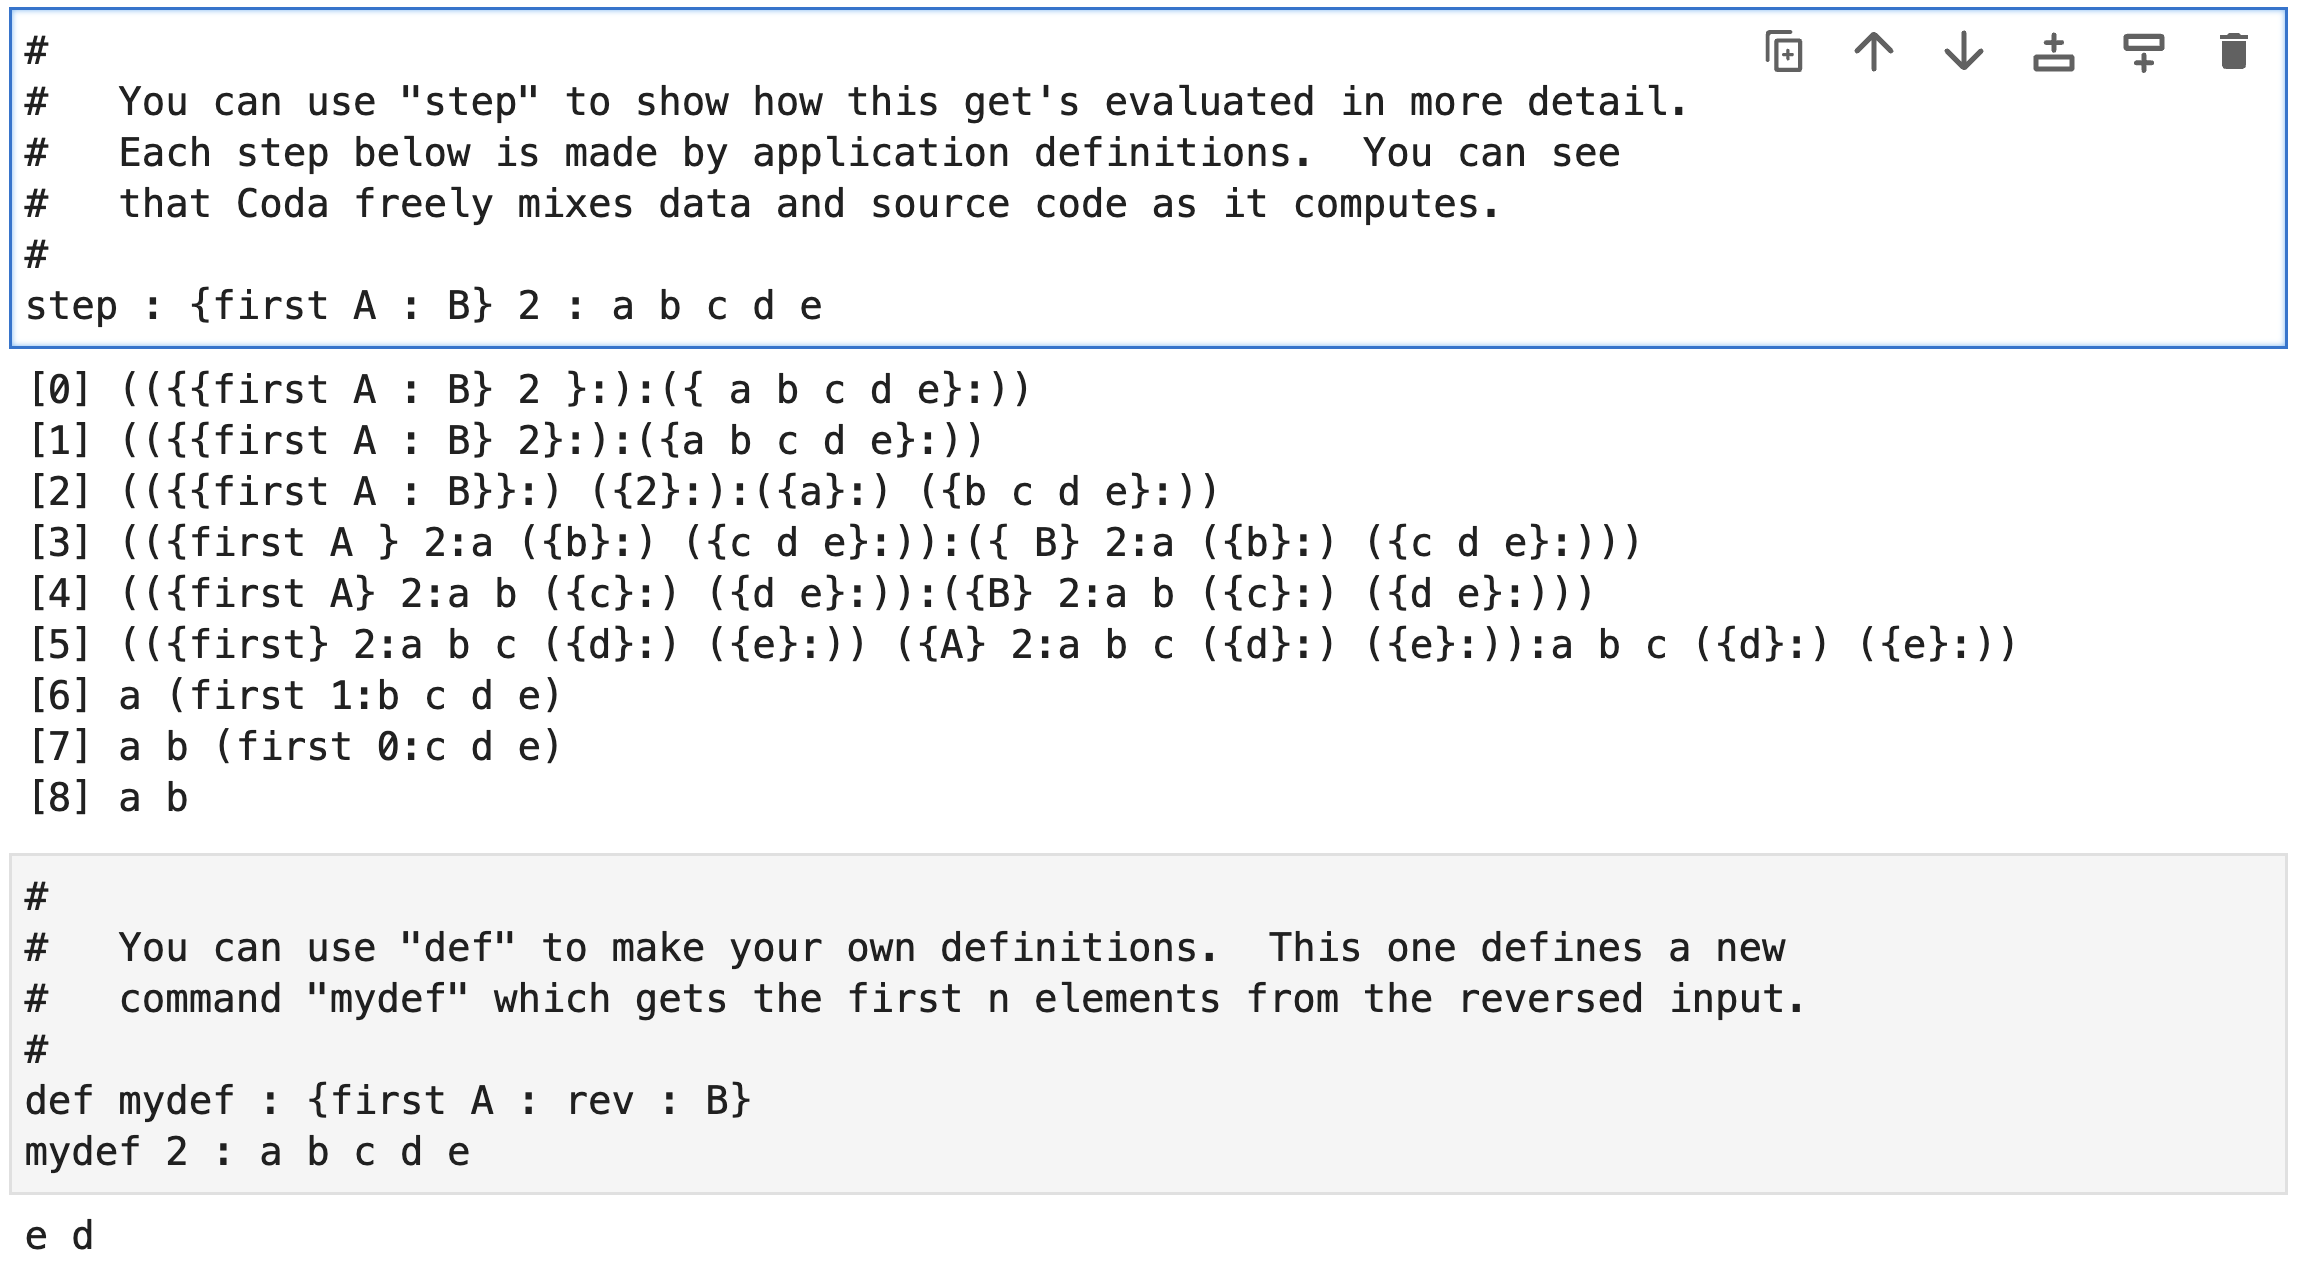
\includegraphics[width=0.9\textwidth]{language_examples.png}
\caption{{\it Example of a coda language expression where each step is in the computation is displayed, showing that language data wrapped 
in curly braces freely mixes with any other data as the computation proceeds.}}
\end{figure} 
Figure 1 shows an evaluation of the language expression ``step : \{first A : B\} 2 : a b c d e''.  In general, {\it evaluation} means applying 
definitions in some unspecified order.  The {\bf step} definition causes the evaluation to be displayed at each step, showing language expressions 
mixing with other data as the evaluation proceeds.  As shown, the language includes definitions which allow you to create definitions as in the 
example ``def mydef : {first A : rev : B}'' which takes ``input'' (B), reverses the order and then selects the first $n$ items in the reversed sequence 
where $n$ is determined by the ``argument'' A.  

     The language is intentionally minimalist - essentially it is a wrap around the two foundational operations of the algebra of data.
Only the characters ``{\bf():\{\}=*/\ }" have language significance.  There are no reserved keywords or 
special syntax for variables, functions, classes or exceptions.  The language is unusual in that any byte sequence is a valid language expression.  
This means that we do not have to specify an alphabet or even define valid and invalid syntax.  There is no such thing 
as invalid syntax.  This also has the benefit that the source code for the compiler and parser is small enough to be easily read and understood by 
humans \cite{github}.

\section{Proof and Computation}

     As noted in Section 2, coda is both a formal system and a computational system.  As a formal system, the `sentences` of the formal system 
are the pure data and the valid `rules of deduction' are to apply the context $\delta$ to any part of some starting data $A_0$ in any chosen order and any finite 
number of times.   This results in a sequence $A_0,A_1,\dots,A_n$.  One has a different sequence depending on the choices, but equations (1) and (2) 
guarantee that $A_0=A_1=\dots=A_n$ in all cases.  In this framework, the difference between a proof 
and a computation is merely in the strategy of when to apply $\delta$ to which coda within some $A_j$.  For most results here, we are using 
a simple computation-oriented strategy of repeated applying $\delta$ everywhere possible and stopping if data in $A_0,A_1,\dots,A_n$ repeats. 
Figures X shows an example of this strategy.   Figure Y shows the same strategy again, this time in a situation 
where the sequence does not, of course, converge and showing how undecided data is used to represent unfinished parts of a
computation or undefined results such as `the last natural number.' 

\begin{figure}[h]
\centering
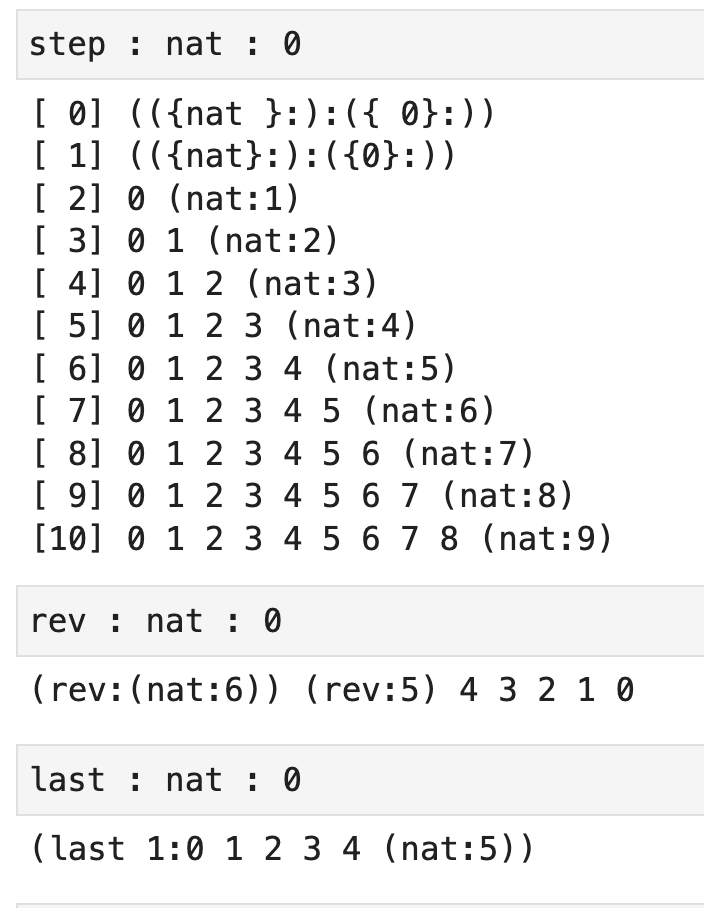
\includegraphics[width=0.7\textwidth]{nat.png}
\caption{Except from a coda session in a jupyter notebook\cite{github}.}
\end{figure} 

    The results obtained here mostly come from the above simple strategy, which we refer to as `evaluation.'  
We expect that there is much to be gained from a much more sophisticated evaluation strategies 
where one optimizes and where and when $\delta$ is applied and where the equally valid $\delta(A)\mapsto A$ moves are included as well 
as $A\mapsto\delta(A)$, but this is mostly unexplored territory as of this writing.  Coda has a couple of unusual and attractive computational properties.  
Since $\delta$ is a partial function, it cannot `loop', by definition.  This means that an evaluation sequence $A_0,A_1,\dots$ may continue forever, 
but each step in the sequence is guaranteed to terminate.  Also, pure data becomes like an executable in the sequence so computations or 
proofs can always be saved at any point and resumed later.  

\section{Spaces}

     Since the algebra of data is common to all pure data, we expect this to be a common structure shared 
 across essentially all mathematical situations.  In this sense, the algebra is analogous to category theory 
 in mathematics.  Here we take a few steps towards developing the algebra, aiming at the most natural 
 way of specifying collections of data of interest called `spaces' and their associated `morphisms.'  First, a few 
 preliminary definitions.  
 \begin{itemize}
 \item $A$ is {\it idempotent} if $A:A:X=A:X$ for all data $X$.
 \item $A$ is {\it distributive} if $A:X\ Y=(A:X)\ (A:Y)$ for all $X$, $Y$.
 \item $A$ is {\it abelian} if $A:X\ Y=A:Y\ X$ for all $X$, $Y$.
 \end{itemize}
 With the algebra of data in mind, any fixed data $A$ defines a collection 
\begin{equation}\label{eqn}
A:X
\end{equation}
where $X$ can be any data.  We can refer to this collection by specifying $A$ and we say that $(A:X)$ {\it belongs to} $A$.  Naturally, 
if $(A:X)$ and $(A:Y)$ belong to $A$, we want $(A:X)\ (A:Y)$ to also belong to $A$.  This is nicely guaranteed if 
we require  
\begin{equation}\label{eqn}
A : (A : X)\ ( A: Y) = A : X\ Y 
\end{equation}
for all data $X$ and $Y$.  Thus, we have the definition of a {\it space}.  Given two spaces $A$ and $B$, if 
distributive data $F$ satisfies 
\begin{equation}\label{eqn}
F : A : X = B : F : X,
\end{equation}
then $F$ is a mapping from $A$ to $B$ where the distributivity of $F$ guarantees that $F$ respects sequences.  
In this situation, we say that $F$ is a {\it morphism} from space $A$ to space $B$.  In the case where $F$ 
is a morphism from space $A$ to $A$, we just say that $F$ is a `morphism of $A$.'  With abuse of pure data 
equality, we say that $F$ is a morphism from $A$ to $B$ if $F*A=B*F$ where $A*B:X$ is defined to be $A:B:X$.  
Each space has a special element $(A:)$ which we call the {\it neutral data} or the {\it neutral element} of a space.  
If $A$ is a space and if space $B$ neutralizes each $A:X$ in the sense that 
\begin{equation}\label{eqn}
A : (A:X)\ (B:X) = A : (B:X)\ (A:X) =  (A:)
\end{equation}
then we call $B$ an {\it anti-space} of $A$. 

Table 3 shows examples of a spaces and their corresponding morphisms.  
\begin{table}
\begin{tabular}{| l | l | l | l | l |  }
Space & Action & Data &  $F*Space=Space*F$ \\
\hline 
pass & A$\mapsto$A & All data & F distributive \\
null & A$\mapsto$ () & () only & F such that F:X=() \\
first & a A$\mapsto$ a & Single atoms &  F(a) for atom a \\ 
bool & A$\mapsto$() $or$ (:) & () or (:) &  F preserving logic \\
type n & A$\mapsto$ (n:3) (n:5) & Natural numbers &  (type n)$*$F$*$(type n) for any F \\
sum n & (n:5) (n:3)$\mapsto$ (n:8) & Natural numbers &  $F(n_1+n_2)=F(n_1)+F(n_2)$ \\
prod n & (n:5) (n:3)$\mapsto$ (n:15) & Natural numbers &  $F(n_1*n_2)=F(n_1)*F(n_2)$ \\
sort n & (n:5) (n:3)$\mapsto$ (n:3) (n:5) & Natural numbers & $n_1\le n_2 \implies F(n_1)\le F(n_2)$ \\
set n & (n:5) (n:3)$\mapsto$ equiv. classes & equiv. classes & F preserving classes \\
Sum n & $F_1\ F_2\dots F_n\mapsto F_1*\dots *F_n$ & Linear maps $n\mapsto n$ & Functorial \\
Sum & $F_1\ F_2\dots F_n\mapsto F_1*\dots *F_n$ & Linear maps  & Functorial \\
Space & $A\mapsto S_1 S_2\dots S_n$ & Spaces & ${\rm Space}*F*{\rm Space}$ for any $F$\\
Mor & $F_1\ F_2\dots F_n\mapsto F_1*\dots *F_n$ & Morphisms & Functorial \\
\hline
\end{tabular} 
\caption{\label{Spaces in Coda}}   
\end{table}
In general, one can think of a space as doing two things:  a) selecting data of interest and b) defining how 
a finite sequence of selected data are combined to make new data in the space.  
The situation with (type n) is typical.  The space (type n) constructs natural numbers from it's ``input'' if possible, 
discarding anything that can't be converted to natural numbers represented as codas like (n:5).  (type n) is 
distributive and, therefore, idempotent so for instance type n : 5 = (n:5) = type n: (n:5) 
The data that (type n) selects is finite  
sequences of natural numbers such as (n:2) (n:1) (n:5).  Since (type n) is distributive, the endomorphisms 
of (type n) are sequence preserving arbitrary functions from naturals to naturals.    
The data (sum n) is also a space, selecting the same sequences of  natural numbers as (type n), but combining 
sequences with addition so that sum n : (n:2) (n:1) (n:5) is equal to (n:8).  The endomorphism of (sum n) 
must satisfy $(sum n):F:X = F:(sum n):X$ which is exactly the condition that $F$ be linear in the ordinary sense. 
Endomorphisms of (sort n), on the other hand, must satisfy $(sort n):F:X=F:(sort n):X$ which is also just 
the condition that $F$ be an order preserving function in the order theory sense.  

     It seems promising to create an abstract theory of spaces with different additional properties.  For 
 example, 
\begin{itemize}
\item A space with an anti-space is a {\it pure group}.
\end{itemize}
The name is justified because the set $\{G:X | $X$\ is\ pure\ data\}$ 
is a group in the ordinary sense if associative composition is defined to be $(G:X)\times(G:Y)\rightarrow G:(G:X)\ (G:Y)$, so that   
$(G:)$ the identity, and where $(G^{-1}:X)$ is the inverse of $(G:X)$ assuming $G^{-1}$ is the promised anti-space of $G$.  

    Although the theory of spaces and morphisms clearly has the flavor of category theory, there are 
also drastic differences.  In category theory, morphisms can be composed only if their domains and co-domains 
agree.  In coda, on the other hand, {\it any} data $F$, $G$ and $H$ can be composed via 
$X\rightarrow H:G:F:X$.  For example, in Table 3, if $F_1,F_2,\dots,F_n$ are in the space 
Hom Sum, $F_1$ is a morphism from some linear space $A_1$ to some linear space $B_1$, $F_2$ is a 
morphism from some linear space $A_2$ to some linear space $B_2$, etc.  The product $F_1*F_2*\dots *F_n$ 
is always defined.  When domains and codomains don't agree in the category theory sense, one just gets 
$F_j:A=()$ making the whole product empty, since the $F_j$ are all distributive.  Another major structural difference 
is the relationship between spaces and morphisms.  In the theory of spaces, the morphisms between space 
$A$ and space $B$ are determined by $A$ and $B$ already.  In categories, the situation is different in the 
sense that there is a choice of morphisms.  For example, nothing prevents one from defining a category 
of real vector spaces with arbitrary functions as morphisms.  

     Another interesting possibility related to spaces might be called ``mathematical machine learning."  A simple 
example is illustrated in Figure X where we imagine that we have become interested in two different 
collections of mathematical objects each just consisting of finite sequences of ``hydrogen atoms" (:).  
\begin{figure}[h]
\centering
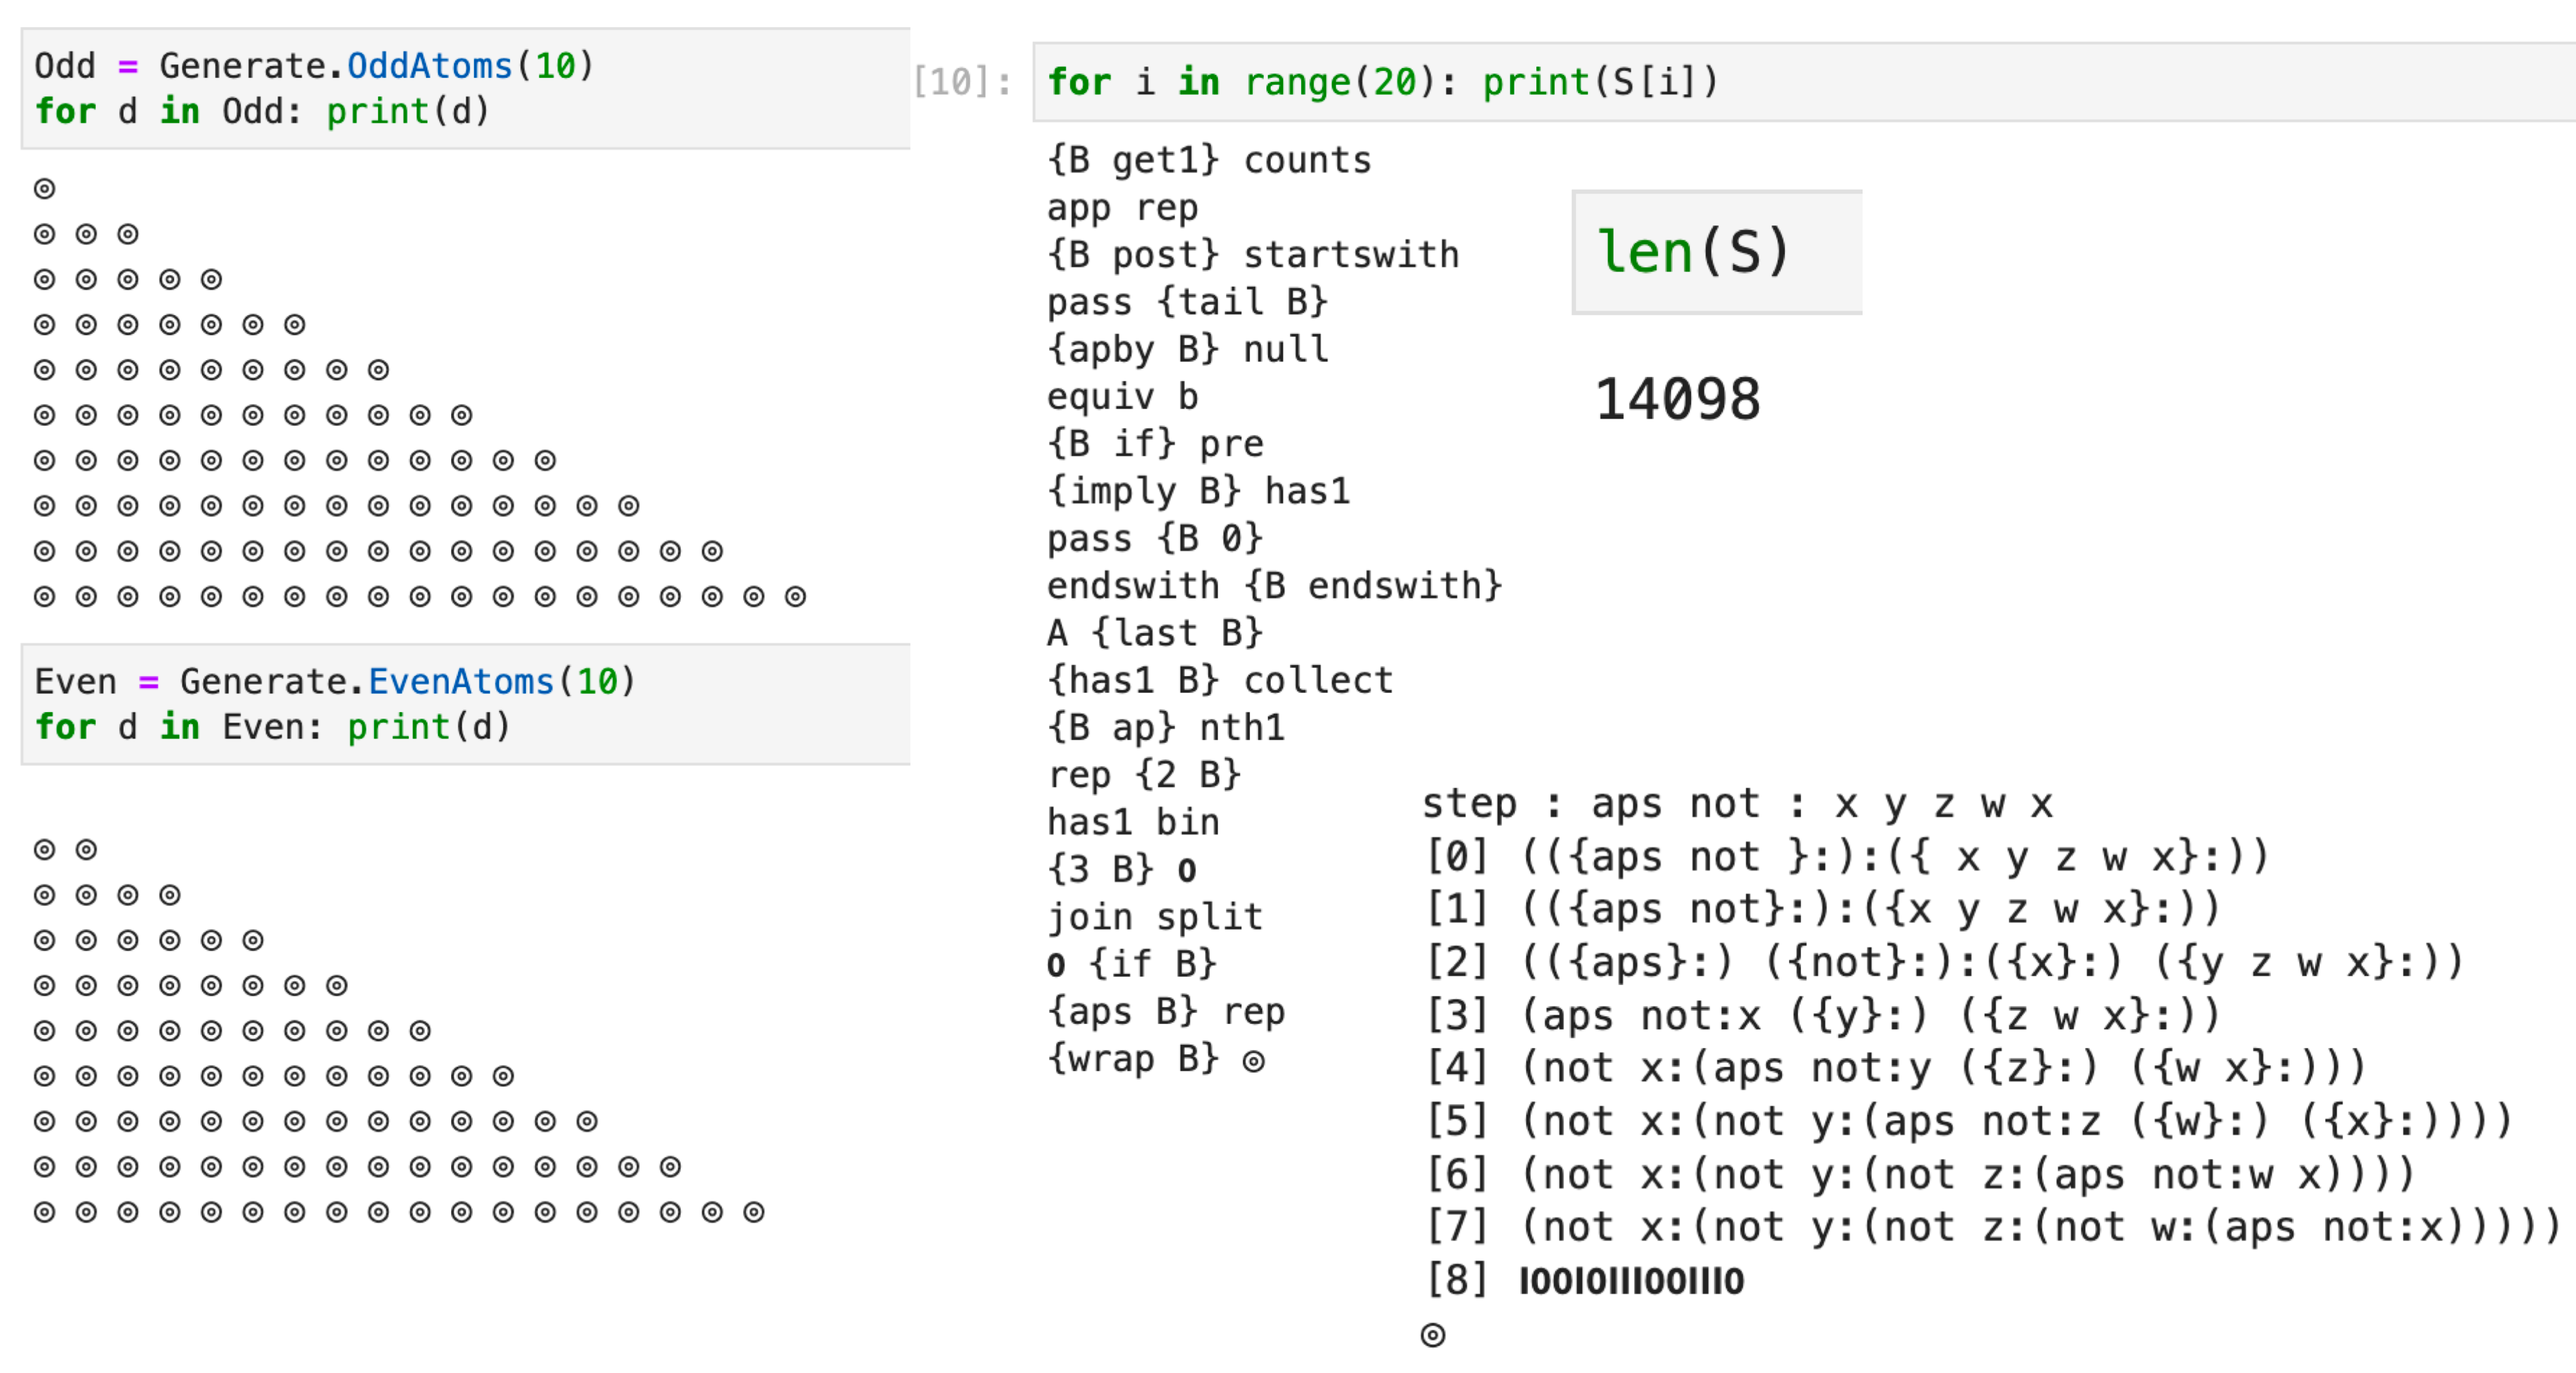
\includegraphics[width=0.7\textwidth]{machine_learning.png}
\caption{Except from a coda session in a jupyter notebook\cite{github}, abs not etc.}
\end{figure} 
The difference between the two collections is that one has an odd number of atoms in each sequence and 
the other has an even number.  We proceed by searching for data $A$ that succeeds in classifying 
the two samples in the sense that $A:X$ have different logical values for the two collections.  The search 
succeeds and finds, for instance, that the data {\bf aps not} is true for one sample and false for the other.  
Some features of the solution are interesting.
\begin{itemize}
\item The solution is clever.  It combines a combinatorial operator {\bf aps} with a logical operator {\bf not} 
in a way that I did not think of before doing the search.  {\bf aps} is the combinatorial operator that turns 
binary operations like (+ A:B) to the corresponding sequential operator summing $b_0+b_1+\dots$ for however
many codas are in $B$ and {\bf not} is logical negation for coda logic.  {\bf not:B} is true if B is false and 
false if B is true.  
\item The solution generalizes.  {\bf aps not} selects data with an even number of atoms in all cases, 
not just when applied to sequences of (:).  
\item Although {\bf aps not} is not quite a space, the minor modification {\bf bool * (aps not)} is a space
in the above sense, and so classifying data of interest has given us both a solution and a ``new'' mathematical structure. 
\item The morphisms of the space {\bf bool * (aps not)} are interesting.  They are the functions 
which preserve atomic parity of data. 
\end{itemize}
Although this is very much a first toy example, this appears to be a general strategy of interest.  

\section{Is Mathematics Consistent?}

     We have defined empty data to be {\it true} and atomic data to be {\it false}.  But since data 
cannot be both true and false, we have seemingly proven that coda is consistent, seemingly 
in contradiction with G\"{o}del's second incompleteness theorem.  To explore this issue  
express the consistency of coda directly in coda.  The following data 
\begin{equation}\label{eqn}
{\rm ap\ \{xor\ (coda:B) : (not:coda:B) \} : allByteSequences :} 
\end{equation}
logically expresses the consistency of coda in the logic of coda.  The definition `coda' maps 
byte sequences to data via the onto mapping $s\mapsto (s:)$.  This means that $({\rm coda}:s)$ and 
$({\rm not}:{\rm coda}:s)$ will be evaluated for each byte sequence $s$ and if they ever have the same logical 
value, the overall value of (11) is false.   Although each application of ${\rm xor}\ ({\rm coda}:B) : ({\rm not}:{\rm coda}:B)$ 
is true in (11), we cannot quite conclude that (11) is true because (allByteSequences:) will   
eventually produce the entire byte sequence (11), which will then recursively get evaluated 
without limit.  Thus, we have the situation where (11) is equal to 
\begin{equation}\label{eqn}
() () () () () \dots ()\  (some\ undecided\ data)
\end{equation}
with endless empty sequences concatenated with forever undecided data. 
We know that the undecided data will never produce an atom, but we also know that it will never disappear, 
meaning that (11) never quite becomes equal to (), which is the definition of ``truth.''  This appears 
to be a satisfying answer.  A G\"{o}del-like limitation appears, but, it is also clear that coda 
is essentially consistent in the sense that no actual contradiction can appear, even though we 
cannot prove that the expression ``there will be no contradiction'' is true in the coda internal sense.
Of course, if coda is accepted as a foundation of Mathematics, the same conclusion holds for Mathematics 
in general.  

\section{Paradoxes}

     Here we examine logical paradoxes as a way of stress testing the proposed conception of logic.  
From the coda point of view, any proposition, paradox or not, should be represented as pure data. 
Any pure data can be evaluated in a given context, and do coda must give some sort of answer 
to any such proposition. 

\subsection{G\"{o}del/Liar}

Recall the overall structure of G\"{o}del's second incompleteness argument.  G\"{o}del cleverly constructs a `G\"{o}del sentence' G  
in Peano Arithmetic (PA) that says of itself that G is not provable in PA.  Assuming that PA is consistent in the sense  
that sentences proven in PA are actually, platonically true we proceed to reason outside of PA in human platonic logic as follows. 
\begin{enumerate}
\item Suppose that G is false;
\item Then G is provable in PA;
\item Since PA consistent by assumption, G is platonically true; 
\item Therefore G is not provable in PA.  $\Rightarrow\!\Leftarrow$;
\item Therefore, G is true. 
\end{enumerate}
Thus, we conclude that G is platonically true, but G is not provable within PA.  

In coda, data $X$ is provable if and only if $X=()$, so we only have to evaluate a `G\"{o}del coda' $G?$ 
with definition $G?\mapsto {\rm not}:G?$.   This definition is established by 
\begin{itemize}
\item let G : not : G? 
\end{itemize}
in the coda language. 
Evaluating $G?$ a few times, we conclude that $G?$ is equal to the undecided data 
\begin{equation}\label{eqn} 
{\rm (not:(not:(not:(not:(not:(not:(not:(not:(not:(({not}:):({G?}:)))))))))))}
\end{equation} 
which is neither true (empty) nor false (atomic).  
Since further evaluation of (13) just produces more of the same, $G?$ is an example of data which is {\it undecidable}.   At this point, 
G\"{o}del's argument could be repeated to conclude that $G?$ is platonically {\it true}, but unprovable in coda.  This seems less 
appealing than in G\"odel's argument, just because the self-referential source of the problem is so much more direct.  An alternative 
is to adopt coda logic platonically and just consider $G?$ to be neither true nor false.   

\subsection{Berry} 

     One possible attitude about, say, the liar paradox, is to avoid a mathematical paradox by just excluding 
the sentence  from Mathematics.  After all, not all English sentences make sense mathematically, and perhaps the liar paradox is just another such sentence.  This point of view becomes less convincing with Berry's paradox\cite{berry} since 
 is seems like a legitimate mathematical problem.  
 \begin{itemize}
 \item {\it Let N = The smallest positive integer not definable in less than twelve words.} 
 \end{itemize}
The problem is this.  Surely, for any positive integer $N$, $N$ either is or isn't definable in less than twelve words.  
There is, therefore, a smallest such integer.  But if such an integer exists, we have succeeded in defining it in 
less than twelve words.  This is a contradiction.  

     To examine the situation in coda, we can proceed directly.  Consider the coda language expression
\begin{equation}\label{eqn}
{\rm maxint : ap\ \{coda:B\} : codes : 32}
\end{equation}
where `codes : 32' produces all character strings with length 32 or less.  Since the length of (X) is 33 characters, 
this is a well defined computation resulting in an integer\cite{unrealistic}.  However, if 32 is replaced by 34, 
`codes : 34' will eventually produce the string `max : ap \{coda:B\} : codes : 34' and the expression will 
recursively remain undecided no matter how it is evaluated.  The situation is the same as in Section 8.  

\subsection{Yablo}

     Although the Liar and Berry paradoxes are self-referential, having self-referential sentences does not 
capture the problem.  This was shown by Yablo\cite{Yablo} who considers the following infinite sequence of non-self referential 
sentences
\begin{itemize}
\item Let $Y_1$ be $true$ if $Y_i$ is false for all $i>1$.
\item Let $Y_2$ be $true$ if $Y_i$ is false for all $i>2$.
\item Let $Y_3$ be $true$ if $Y_i$ is false for all $i>3$.
\item \dots
\end{itemize}
Suppose that $Y_n$ is true for some $n$.  Then all sentences greater than $Y_n$ are false.  But this means 
that all sentences greater than $Y_{n+1}$ are also false, which means that $Y_{n+1}$ is true, contradicting 
the assumption that $Y_n$ is true.  Thus, $Y_n$ cannot be true for any $n$.  But if all $Y_i$ are all false, then  
$Y_0$ is true.  This is a contradiction.  

     As in the previous cases, we can proceed concretely.  Introduce a definition for Yablo as follows. 
\begin{itemize}
\item def Yablo : \{ap not : Yablo : skip 1 : nat : B\}
\end{itemize}
so that $({\rm Yablo}:n)$ is true if all of $({\rm Yablo}:n+1)$,\dots are not true.   
\begin{figure}[h]
\centering
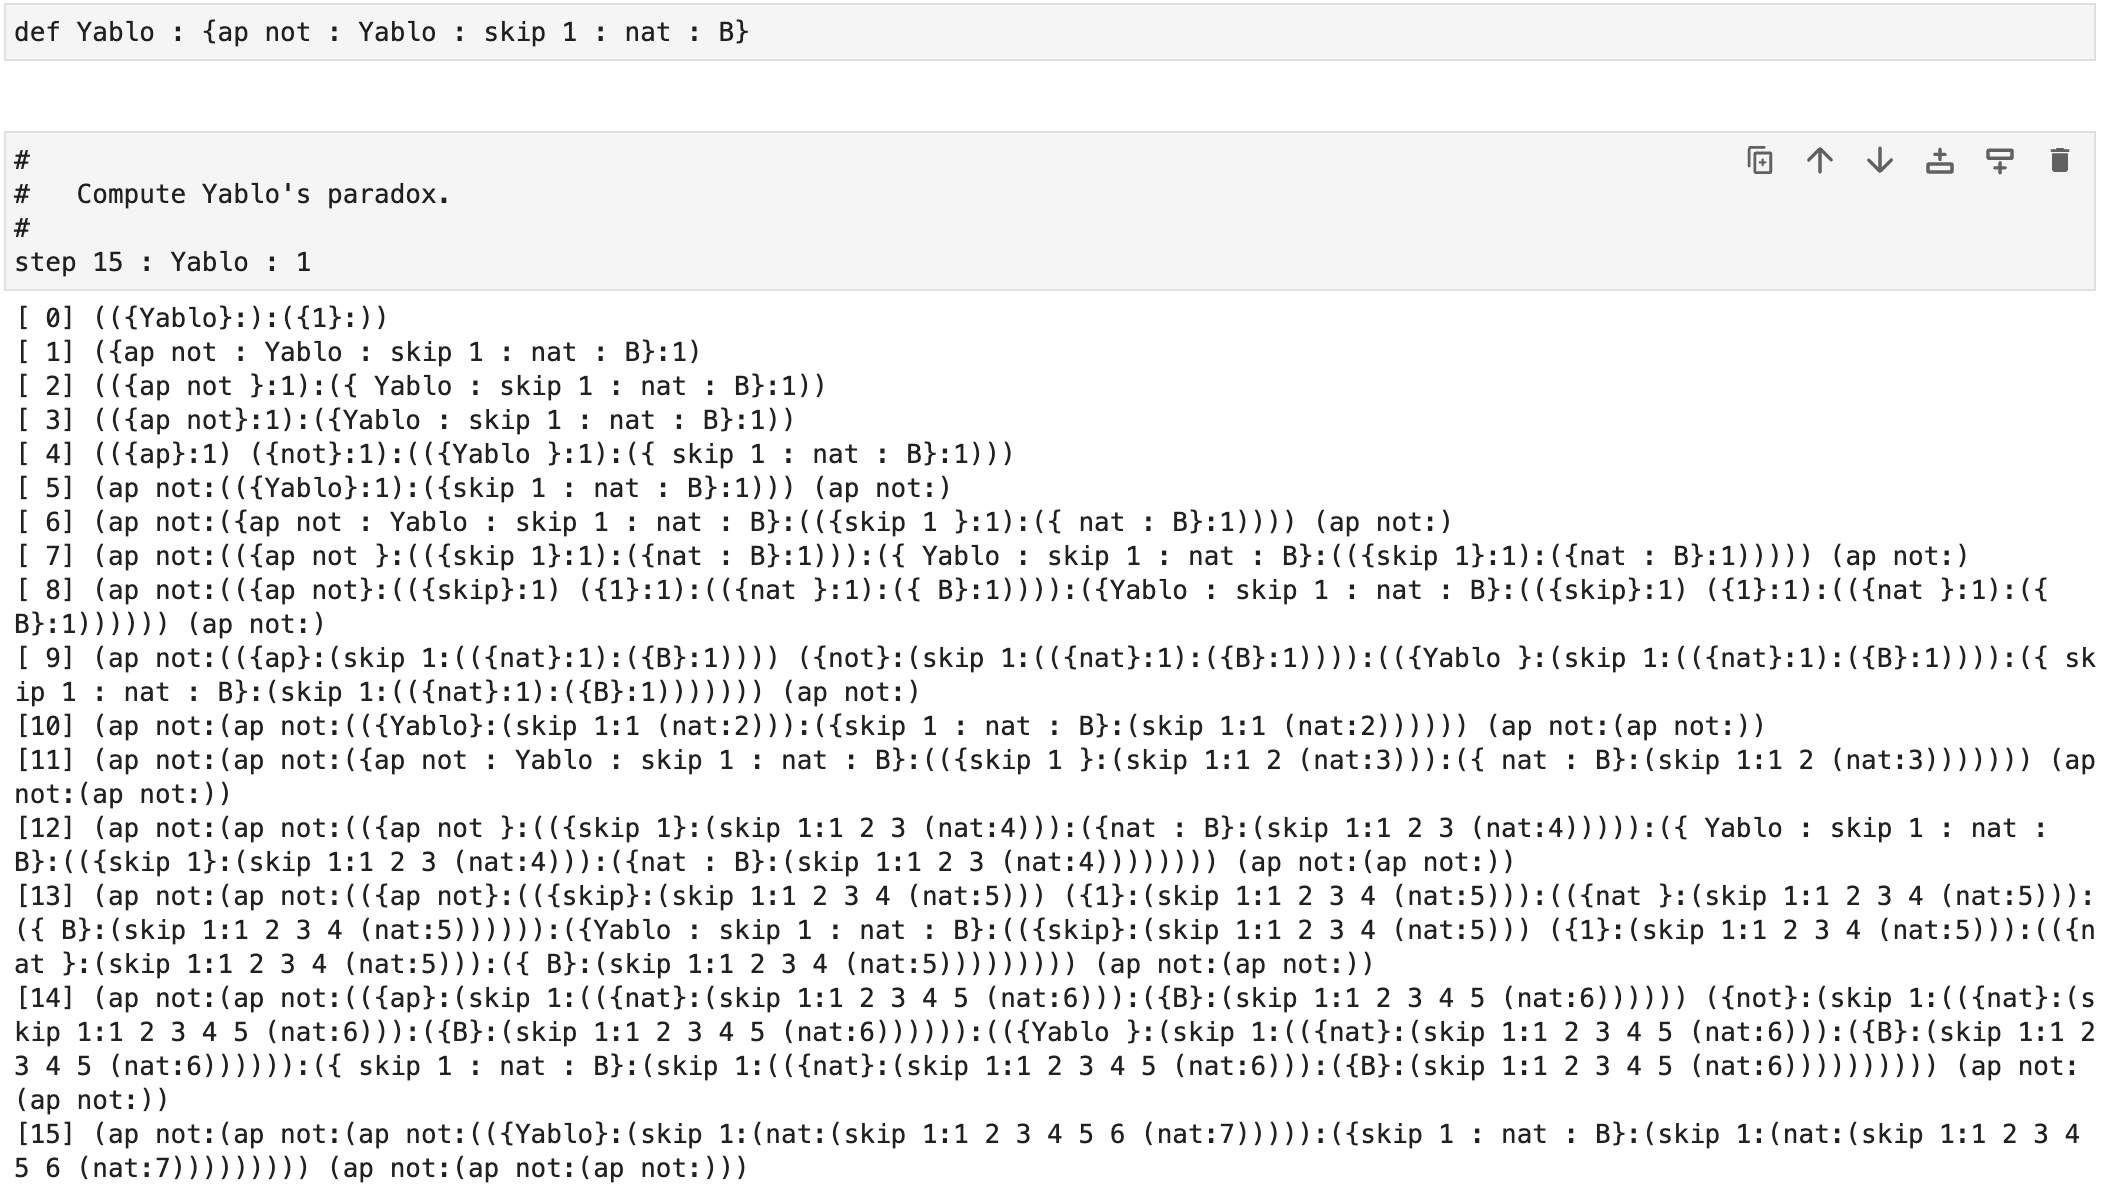
\includegraphics[width=0.9\textwidth]{Yablo.png}
\caption{{\it Evaluation of $Y_1$ in coda.}}
\end{figure} 
Figure 3 shows the evaluation of $Y_1$ in coda.  The empirical result is that $Y_1$ remains undecided  
to high depth of evaluation.  Although it is not quite as obvious as in the previous cases in this section, 
we expect that $Y_1$ is {\it undecidable} as in the previous cases, indicating in a satisfying way 
that the proposition $Y_1$ undecidable. 

\section{Summary}

%%%%%%%%%%%%%%%%%%%%%%%%%%%%%%%%%%%%%%%%%%%%%%%%%%%%%%%%%%%%%%%%%%%%%%%%
%%% \bibliography{jpsi}
\begin{thebibliography}{10}
\bibitem{logic} Shapiro, Stewart and Teresa Kouri Kissel, "Classical Logic", The Stanford Encyclopedia of Philosophy (Winter 2022 Edition), Edward N. Zalta \& Uri Nodelman (eds.).
\bibitem{github} Source code in github. 
\bibitem{Godel} 
\bibitem{Yablo} 
\bibitem{Berry}
\bibitem{egg}
\bibitem{aldor}
\bibitem{ZFC}
\bibitem{HOTT}
\end{thebibliography}
%%%%%%%%%%%%%%%%%%%%%%%%%%%%%%%%%%%%%%%%%%%%%%%%%%%%%%%%%%%%%%%%%%%%%%%%
\end{document}
